\chapter{Pesquisa-ação}
\label{pesquisa_acao}
	\section{Descrição da organização}

		A organização a ser tratada neste trabalho refere-se aos grupos de trabalho das disciplinas de Gestão de Projetos
		e Portfólio (GPP) e Metodologias de Desenvolvimento de Software (MDS), do curso de Engenharia de \textit{Software}
		da Universidade de Brasília.

		A organização trabalha na produção de software com vários projetos, os quais possuem as seguintes características:

		\begin{itemize}
			\item Uso de dados abertos;
			\item Aplicações WEB e aplicativos \textit{mobile};
			\item Equipe composta de dois times:
				\subitem 1 time de desenvolvimento;
				\subitem 1 equipe de gerência;
			\item Equipes pequenas e inexperientes;
			\item Prazo fixo;
		\end{itemize}

		\subsection{Objeto da ação}

		Para a realização da pesquisa-ação será considerado um projeto em andamento da organização que possui as seguintes características:


		\begin{itemize}
			\item Aplicativo \textit{mobile};
			\item Equipe composta de dois times:
				\subitem 1 time de desenvolvimento com 6 pessoas;
				\subitem 1 equipe de gerência com 6 pessoas;
			\item Membros inexperientes na tecnologia.
			\item Uso de metodologia ágil;
			\item Quantidade de \textit{Sprints}: 7;
			\item Tamanho da \textit{Sprint}: 1 semana;
			\item Dedicação parcial do time, visto que trata-se de uma disciplina.
		\end{itemize}

	\pagebreak


\section{Diagnóstico}

	O diagnóstico realizado para ver a situação atual do projeto selecionado para o estudo consistiu na análise 
	dos gráficos de \textit{Burndown} das quatro primeiras \textit{Sprints} e na aplicação de um questionário para o 
	time de desenvolvimento.
	
	\subsection{Análise dos gráficos de \textit{Burndown}}

	Para as quatro primeiras \textit{Sprints} é possível ver nas Figuras \ref{fig:burndown0}, \ref{fig:burndown1}, \ref{fig:burndown2}
	\ref{fig:burndown3} que os pontos realizados não correspondem a pontuação total planejada para a \textit{Sprint}. 
	Assim é possível ver que que nem todas as histórias alocadas foram entregues, o que significa que houve atrasos nas entregas.

	O acompanhamento do \textit{Burndown} por \textit{Sprint} auxiliou na visualização da distribuição do trabalho dentro da \textit{Sprint}.
	Assim foi possível ver, por exemplo, que nas \textit{Sprints} 0 e 1 o time demorou para começar a trabalhar, o que pode ter sido uma causa do atraso. Dessa forma, impactando nas \textit{Sprints} seguintes.

	\begin{figure}[!h]
	\begin{minipage}[b]{0.5\linewidth} 
	\centering
	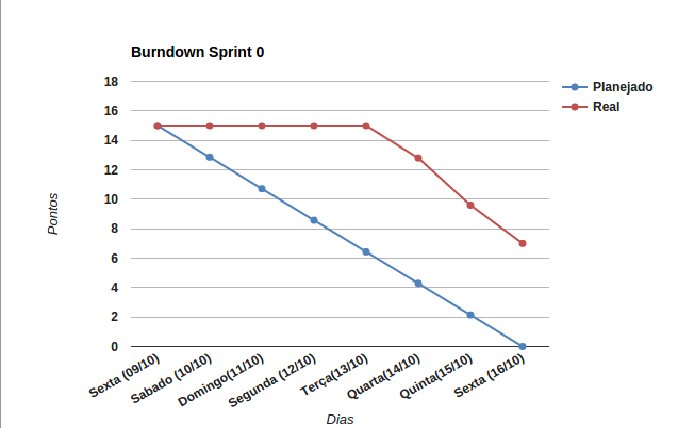
\includegraphics[scale=0.5]{figuras/burndown_sprint0.png}
	\caption{Burndown da Sprint 0.}
	\label{fig:burndown0}
	\end{minipage}
	\hspace{0.5cm} 
	\begin{minipage}[b]{0.5\linewidth}
	\centering
	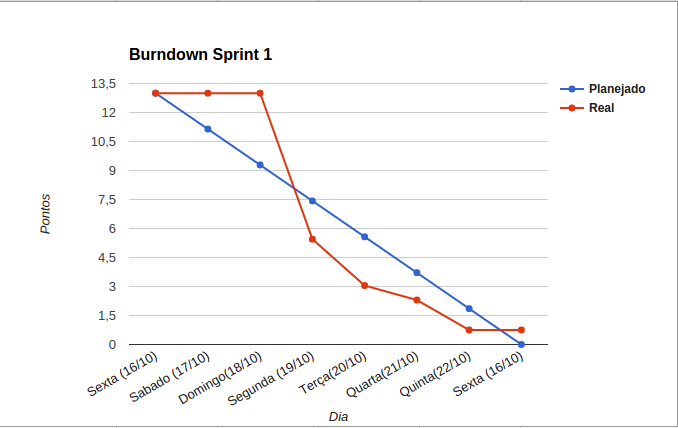
\includegraphics[scale=0.5]{figuras/burndown_sprint1.png}
	\caption{Burndown da Sprint 1.}
	\label{fig:burndown1}
	\end{minipage}
	\end{figure}
	
	\begin{figure}[!h]
	\begin{minipage}[b]{0.5\linewidth} 
	\centering
	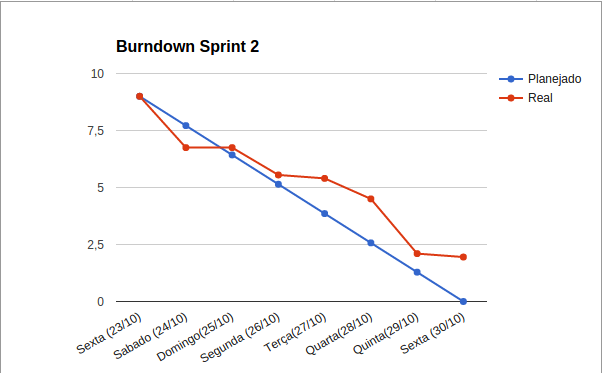
\includegraphics[scale=0.5]{figuras/burndown_sprint2.png}
	\caption{Burndown da Sprint 2.}
	\label{fig:burndown2}
	\end{minipage}
	\hspace{0.5cm} 
	\begin{minipage}[b]{0.5\linewidth}
	\centering
	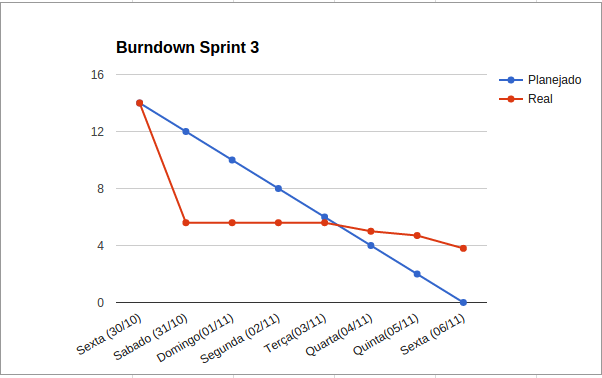
\includegraphics[scale=0.5]{figuras/burndown_sprint3.png}
	\caption{Burndown da Sprint 3.}
	\label{fig:burndown3}
	\end{minipage}
	\end{figure}
	
	\pagebreak


	\subsection{Questionário}

	A fim de coletar dados sobre a percepção dos membros sobre possíveis aspectos que afetaram a entrega nos prazos foi aplicado
	um questionário ao time de desenvolvimento que se encontra no apêndice \ref{apendice:questionario}.



	\section{Planejamento da ação}

		SOMMERVILLE (2007) destaca que a medição de software preocupa-se com a derivação de um valor numérico ou o perfil para um atributo de um componente de software, sistema ou processo. Comparando esses valores entre si e com os padrões que se aplicam a toda a organização, pode-se tirar conclusões sobre a qualidade do software ou avaliar a eficácia dos métodos, das ferramentas e dos processos de software. Como dizia Tom de Marco (1982), "Não se pode gerenciar o que não se pode medir".

		Softwares podem ser medidos (ou estimados) de diversas formas, como tamanho, custo e esforço. E, para a medição de um produto, podem ser colhidas diferentes métricas. Por exemplo, para a medição de tamanho na etapa de levantamento de requisitos, pode-se utilizar como métrica o número de requisitos especificados. Já na fase de projeto, o tamanho pode ser medido em função do número de classes e, na fase de codificação, a partir no número de linhas de código fonte.

		http://www.devmedia.com.br/artigo-engenharia-de-software-21-metricas-de-software/15776

		https://www.assembla.com/spaces/procsw/documents/d92WTA434r36xHeJe5cbLA/download/d92WTA434r36xHeJe5cbLA

		BASSI (2012) cita a metodologia Lean como sendo distribuída nos princípios de eliminar o desperdício, amplificar o aprendizado, adiar comprometimentos e manter a flexibilidade, entregar rápido, tornar a equipe responsável, construir integridade e visualizar o todo. O princípio de eliminar o desperdício foca no sentido de que o desperdício em si pode acontecer em vários sentidos, entre eles: dinheiro, recursos, tempo, esforço e espaço. Cada etapa e atividade realizada no processo devem contribuir para que seja possível construir um produto final com menos custo, mais rapidez e com qualidade.

		Para esse trabalho foram escolhidas três métricas principais: esforço, tamanho e tempo. A métrica tamanho, como já foi citado, pode ser alcançada de diversas formas. Para o contexto do trabalho analisaremos o tamanho realizando a contagem de número de linhas de código que, por sua vez, auxiliará a estimar o esforço a ser considerado para a obtenção de um produto a ser desenvolvido. O tempo estudado será aquele estimado a se realizar determinada tarefa.

\section{Execução da ação}
\section{Avaliação da ação}